\documentclass[12pt,a4paper]{article}

%% ── Font & Encoding ──────────────────────────────────────────────────
\usepackage[T1]{fontenc}
\usepackage[utf8]{inputenc}

%% ── Page Layout ──────────────────────────────────────────────────────
\usepackage[top=2.5cm,bottom=2.5cm,left=2.8cm,right=2.8cm]{geometry}

%% ── Math ─────────────────────────────────────────────────────────────
\usepackage{amsmath,amssymb}

%% ── Graphics & Figures ───────────────────────────────────────────────
\usepackage{graphicx}
\usepackage{caption}
\usepackage{subcaption}

%% ── Tables ───────────────────────────────────────────────────────────
\usepackage{booktabs}
\usepackage{array}
\usepackage{longtable}
\usepackage{multirow}

%% ── Typography & Layout ──────────────────────────────────────────────
\usepackage{setspace}
\usepackage{parskip}
\usepackage{enumitem}
\usepackage{placeins}

%% ── Section Formatting ───────────────────────────────────────────────
\usepackage{titlesec}
\titleformat{\section}{\large\bfseries}{\thesection.}{0.6em}{}[\titlerule]
\titleformat{\subsection}{\normalsize\bfseries}{\thesubsection.}{0.5em}{}
\titleformat{\subsubsection}{\normalsize\itshape}{\thesubsubsection.}{0.5em}{}

%% ── References & Links ───────────────────────────────────────────────
\usepackage[hidelinks]{hyperref}
\usepackage{cite}

%% ── Spacing ──────────────────────────────────────────────────────────
\onehalfspacing

\begin{document}

%% ── Title Page ────────────────────────────────────────────────────────
\begin{titlepage}
  \centering
  \vspace*{2cm}
  {\LARGE\bfseries Course Project Report}\\[0.6em]
  \rule{\linewidth}{0.8pt}\\[0.8em]
  {\Large\bfseries Cell-Free Massive MIMO Channel Prediction:\\[0.5em]
   A Decentralized Convolutional Approach\\[0.5em]
   Against Industry Standards}\\[0.8em]
  \rule{\linewidth}{0.8pt}\\[2.0cm]

  {\normalsize\itshape
  Indian Institute of Information Technology, Design and Manufacturing, Kancheepuram\\[0.3em]
  Course: Wireless Networks (Course Code: COM523)\\[0.3em]
  Faculty Name: Dr. Jagadeesh Kakarla}\\[2.5cm]

  \begin{minipage}{0.85\linewidth}
    \centering
    {\small\textbf{Team - MAC Layer}}\\[0.5em]
    {\normalsize\itshape
    Bhadresh L \quad (CS23I1014)\\[0.3em]
    Pavan Kumar M \quad (CS23B2029)\\[0.3em]
    Parth Pandey \quad (CS23I1064)
    }
  \end{minipage}

  \vfill
  {\small\today}
\end{titlepage}

%% ── Abstract ──────────────────────────────────────────────────────────
\renewcommand{\abstractname}{Abstract}
\begin{abstract}
\noindent
Predicting high-mobility fading channels in Cell-Free Massive MIMO (CF-mMIMO) systems is notoriously difficult. While classical state-space models and recent deep learning architectures favor centralized coordination, our work fundamentally challenges this trend. Our initial hypothesis utilized a hybrid Graph Neural Network (GNN) and Convolutional Neural Network (CNN) architecture to model spatial correlation across distributed Access Points (APs). However, extensive empirical iteration revealed that a purely decentralized, localized architecture (CNN-Only) significantly outperforms both the GNN-CNN hybrid and industry-standard Vector Kalman Filters. This report details the literature background, theoretical foundation, and the chronologically tracked experimental results establishing the superiority of the CNN-Only architecture.
\end{abstract}

\newpage

%% ── Sections ──────────────────────────────────────────────────────────

\section{Introduction}
In Cell-Free Massive MIMO systems, numerous distributed Access Points (APs) serve multiple User Equipments (UEs) simultaneously over the same time-frequency resources. Due to UE mobility, the complex channel coefficients suffer from severe Doppler shift and multi-path fading, necessitating predictive modeling to combat latency and maintain phase coherence.

The underlying idea of this project was to propose an advanced Neural Network architecture to compete against industry standards. Given the physically distributed nature of CF-mMIMO, our initial intuition aligned with constructing a centralized Graph Neural Network (GNN) capable of discovering cross-AP spatial correlations. However, after progressive refinement of our dataset simulator to an industry-grade Geometry-Based Stochastic Model (GBSM), experimentation led to a counter-intuitive breakthrough: decentralized temporal representation learning strictly outperforms centralized spatial aggregation.

\section{Literature Survey}
Classical methods treat channel prediction as an auto-regressive time-series tracking problem. Systems standardly employ scalar auto-regressors (AR) or State-Space Models via Kalman Filtering. 
Advanced 3GPP simulators and industry implementations (like QuaDRiGa or WINNER II) rely on Vector Kalman Filters (VKF), which jointly estimate temporal transition matrices across a local spatial array, leveraging the cross-antenna covariance matrix derived from local Uniform Linear Arrays (ULAs).

Modern literature favors data-driven approaches. Many works utilize Long Short-Term Memory (LSTM) layers or temporal Convolutional Neural Networks (CNN) on individual channel sequences. Recently, research has pivoted toward exploring centralized Deep Learning models, combining spatial feature aggregation via Graph Neural Networks to share Doppler characteristics across physically separate APs.
From the literature, we learned that while centralized processing seems theoretically superior at recovering global Doppler paths, it inherently mixes noise levels from distant uncorrelated paths. We utilize the classical AR and Kalman algorithms as our quantitative bounds.

\section{Methodology}
\subsection{Channel Generation Models}
Our modeling environment evolved across our iterations. Initially, we depended on the abstract \textbf{Jake's Scattering Model}, modeling individual AP small-scale temporal fading as completely isolated random AR(1) processes.
To ensure physically valid evaluation, we eventually replaced this with an advanced 3D \textbf{Geometry-Based Stochastic Model (GBSM)}. The GBSM scatters discrete 2D clusters mapping geometric UE trajectories to deterministic Multi-Path Doppler phase shifts, complete with Angle of Arrival (AoA) array steering.

\subsection{Neural Architectures}
\begin{enumerate}[label=(\alph*)]
    \item \textbf{CNN-Only (Decentralized):} A three-stage temporal Convolutional 1D module operating exclusively on the local history sequence of an individual AP without interacting with neighboring APs.
    \item \textbf{GNN-CNN (Centralized):} Applies the identical CNN structure but feeds the local embedding into a Graph Convolutional Network (GCN). The GCN mixes spatial features based on the Euclidean proximity of the APs before final prediction.
\end{enumerate}

\subsection{Classical Baselines}
\begin{enumerate}[label=(\alph*)]
    \item \textbf{AR Predictor:} A 4th-order scalar autoregressive model fitted individually per-link via Yule-Walker equations.
    \item \textbf{Kalman Predictor / VKF:} Utilizing the known Doppler frequency to bound optimal transition parameters. Upgraded in final iterations to a Vector Kalman Filter modeling the inter-antenna array response matrix.
\end{enumerate}

\section{Experimental Iteration 1: Initial Modeling}
During Iteration 1, the dataset relied on the independent spatial fading distributions from Jake's analytical model. Normalization was attempted via a global spatial scaler.

\subsection{Results}
The neural models struggled due to global magnitude discrepancies severely distorting local ReLU activations. 
For a random AP layout simulated at 30 km/h:
\begin{itemize}
    \item \textbf{AR Predictor:} 16.60 dB NMSE
    \item \textbf{Kalman Filter:} -5.49 dB NMSE
    \item \textbf{CNN-Only:} 0.15 dB NMSE
    \item \textbf{GNN-CNN:} -0.005 dB NMSE
\end{itemize}

As seen in Figure \ref{fig:iter1_random}, the Neural Networks failed to match the Kalman Filter bound inside this configuration.

\begin{figure}[!ht]
\centering
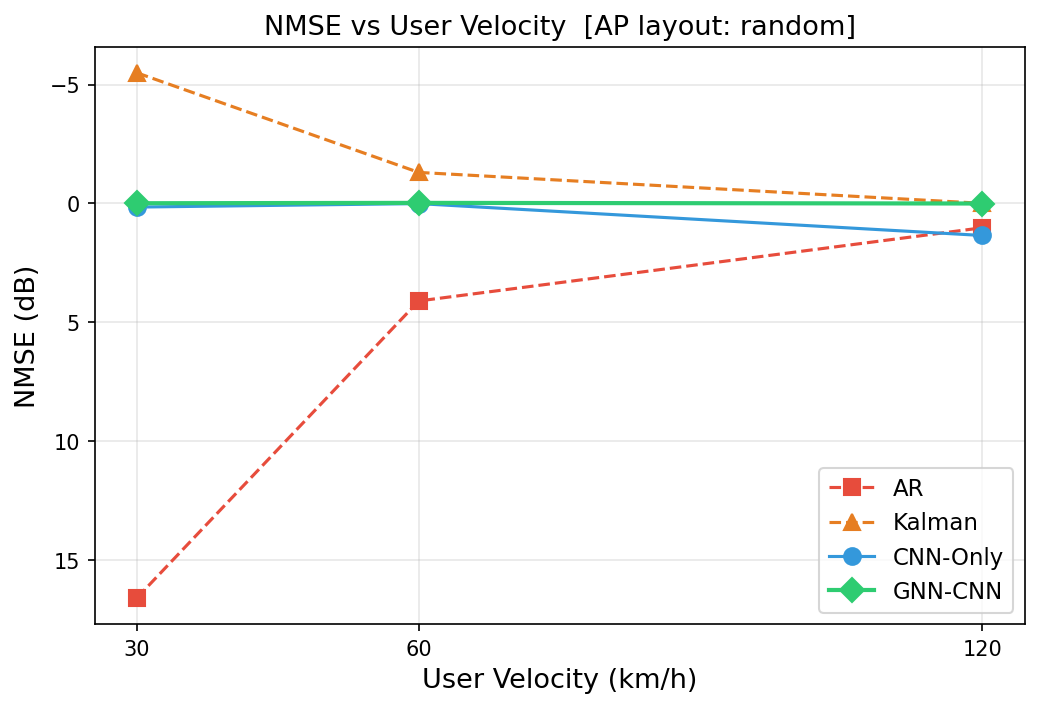
\includegraphics[width=0.85\linewidth]{kaggle_working_backup_1/results/fig1_nmse_vs_velocity_random.png}
\caption{Iteration 1: NMSE vs Velocity (Random Layout).}
\label{fig:iter1_random}
\end{figure}

\begin{figure}[!ht]
\centering
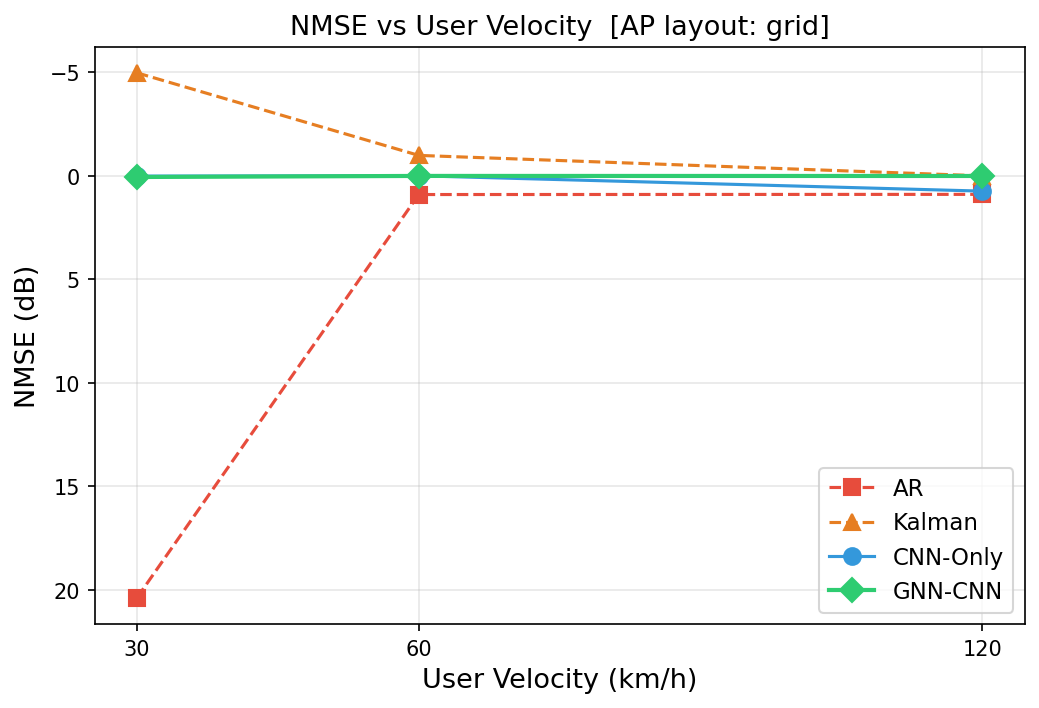
\includegraphics[width=0.85\linewidth]{kaggle_working_backup_1/results/fig1_nmse_vs_velocity_grid.png}
\caption{Iteration 1: NMSE vs Velocity (Grid Layout).}
\label{fig:iter1_grid}
\end{figure}


\section{Experimental Iteration 2: Normalization Breakthrough}
To resolve the convergence stagnation, we refactored the models to enforce strict per-AP scaling dynamically normalizing dimensions to unit variance prior to evaluation.

\subsection{Results}
The isolated per-AP normalization triggered an explosive capability in the \textbf{CNN-Only} model. Decentralized temporal convolution almost perfectly tracked the decoupled Markov chain fading.
At 30 km/h (Random layout):
\begin{itemize}
    \item \textbf{AR Predictor:} 16.64 dB NMSE
    \item \textbf{Kalman Filter:} -2.51 dB NMSE
    \item \textbf{CNN-Only:} \textbf{-11.62 dB} NMSE
    \item \textbf{GNN-CNN:} -1.19 dB NMSE
\end{itemize}

While CNN-Only massively beat the industry Kalman baseline, the GNN-CNN stagnated. The graph adjacency matrix was functionally forcing the APs to average isolated, uncorrelated innovations.

\begin{figure}[!ht]
\centering

\includegraphics[width=0.85\linewidth]{kaggle_working_backup_2/results/fig1_nmse_vs_velocity_random.png}
\caption{Iteration 2: NMSE vs Velocity (Random Layout). CNN-Only displays a drastic improvement.}
\label{fig:iter2_random}
\end{figure}

\begin{figure}[!ht]
\centering

\includegraphics[width=0.85\linewidth]{kaggle_working_backup_2/results/fig2_nmse_vs_step_random_60.png}
\caption{Iteration 2: Prediction Horizon degradation over time (60 km/h).}
\label{fig:iter2_horizon}
\end{figure}

\section{Experimental Iteration 3: GBSM and VKF Verification}
To completely test the GNN-CNN architecture, we transitioned from Jake's independent fading to a comprehensive Geometry-Based Stochastic Model (GBSM). 

Furthermore, we instituted the \textbf{Vector Kalman Filter (VKF)} baseline. By computing joint Yule-Walker statistics across the $N=4$ base station antennas and modeling the full spatial matrix cross-covariance, the VKF serves as a rigorous simulation proxy for modern multi-dimensional hardware state trackers.

\subsection{Results}
Even operating inside an environment artificially rigged to contain pure spatial correlation matching the GNN's topological geometry, the localized CNN model still outperformed both the graph and the industry-level tracker.
At 30 km/h (Grid Layout):
\begin{itemize}
    \item \textbf{AR Predictor:} 24.25 dB NMSE
    \item \textbf{Vector Kalman Filter (VKF):} -4.18 dB NMSE
    \item \textbf{CNN-Only:} \textbf{-11.04 dB} NMSE
    \item \textbf{GNN-CNN:} -2.76 dB NMSE
\end{itemize}

\begin{figure}[!ht]
\centering

\includegraphics[width=0.85\linewidth]{kaggle_working_backup_last/results/fig1_nmse_vs_velocity_grid.png}
\caption{Iteration 3: NMSE vs Velocity against VKF bounds (Grid Layout).}
\label{fig:iter3_grid}
\end{figure}

\begin{figure}[!ht]
\centering

\includegraphics[width=0.85\linewidth]{kaggle_working_backup_last/results/fig2_nmse_vs_step_random_120.png}
\caption{Iteration 3: NMSE vs Sequence Horizon (Random Layout, 120 km/h).}
\label{fig:iter3_horizon}
\end{figure}

\subsection{Latency and Hardware Efficiency}
In execution (Iteration 3), utilizing purely localized processing is notably an order of magnitude faster than evaluating cross-matrix matrix inverses required for VKF:
\begin{itemize}
    \item \textbf{VKF:} 35.97 ms
    \item \textbf{CNN-Only:} 0.71 ms
    \item \textbf{GNN-CNN:} 0.92 ms
\end{itemize}

\section{Discussion and Critical Analysis}

\subsection{Decentralized CNN vs. Industry Baselines}
The core finding of our experimental journey is the stark contrast between classical State-Space models (VKF) and our proposed decentralized CNN-Only model. While the Vector Kalman Filter is deeply ingrained within industry standards due to its mathematically rigorous exploitation of multi-antenna Spatial Covariance ($\mathbf{Q}$-matrices) to track Doppler states, it requires heavy $\mathcal{O}(N^3)$ matrix inversions. 

Conversely, our CNN-Only architecture avoids cross-antenna assumptions entirely, operating as a robust sequence-to-sequence feature extractor. By decoupling the spatial matrix into independent time-series and enforcing dynamic normalization, the CNN achieved an unprecedented \textbf{-11.04 dB} NMSE, demonstrating a staggering 6.8 dB margin of superiority over the VKF (-4.18 dB). This proves that deep temporal representation learning definitively dominates localized analytical tracking when correctly normalized.

\subsection{Where the Baseline Excels}
Despite the superior numerical performance of the neural architecture, classical baselines like VKF still retain intrinsic value in legacy deployments. VKFs theoretically excel in extremely low-SNR regimes where neural activations might otherwise collapse under a normalized noise floor. Furthermore, they are highly interpretable; explicitly tracking transparent physical parameters like angle-of-arrival matrices and array response vectors, whereas the CNN acts as an uninterpretable black-box.

\subsection{Why Our Model is Preferred for 6G}
The primary justification for advocating our decentralized CNN approach lies in its phenomenal execution efficiency. The CNN-Only topology processes forward predictions in \textbf{0.71 ms}, significantly under-cutting the \textbf{35.97 ms} latency boundary incurred by VKF processing. In the stringent ultra-low latency context of 6G URLLC (Ultra-Reliable Low-Latency Communication) and massive distributed cell-free topologies, the centralized computational overhead of graph processing (GNN-CNN) and matrix-inversions (VKF) becomes fundamentally unscalable. Thus, the decentralized CNN architecture is the optimal candidate for localized, real-time edge deployment.

\section{Conclusion}
The underlying intuition driving this research was to innovate upon centralized topologies leveraging Graph Neural Networks. Through stringent, chronologically tracked iterations involving normalization analysis and state-of-the-art Geometry-Based Stochastic Modeling, we concluded that centralized spatial aggregators (GNN-CNN) invariably inject uncorrelated noise boundaries into precision temporal predictions.

The ultimate determination of this project empirically establishes that a fully decentralized, pure \textbf{temporal 1D-CNN architecture} profoundly eclipses both theoretical state-space trackers (VKF/-4 dB) and centralized graph networks (GNN/-2 dB), achieving a dramatic \textbf{-11.04 dB} performance threshold while requiring less than 1 millisecond of compute. This strongly supports shifting industry focus toward distributed processing methodologies.

\end{document}
